\chapter{Forecasting} \label{Chap5}

\section{Overview}

Forecasting extends beyond a fixed origin and therefore cannot use subsequent
FCH\textsubscript{4} observations as context. The experiments follow the five
365-day fixed-origin backtests defined in Chapter~\ref{ChapModels}. Supporting
variables over each evaluation period are treated as known, so the results
measure conditional methane-response forecasting rather than the additional
error involved in forecasting weather or management. Performance is evaluated
against QC-valid observed FCH\textsubscript{4}, not the reconstructed target
series produced in Chapter~\ref{Chap4}.

The benchmark models use different predictor subsets. To avoid repeating a
separate feature inventory for every model, Table~\ref{tab:fc_tabpfn_features}
reports the complete predictor frame used by the TabPFN model. Its best
configuration combines 52 daily environmental and
management drivers with five tower and time indicators. 

% \noindent\textbf{The best-performing forecasting model,}
% TabPFN and TabICL configuration averages three complementary
% TabPFN variants. The first uses all pre-origin observations with a spike
% correction: a classifier estimates whether FCH\textsubscript{4} exceeds the
% tower-specific 95th percentile, and 25\% of the predicted difference between
% spike and non-spike regressors is added to the base prediction. The other
% variants use the most recent 1,095 and 1,460 days, with the latter additionally
% applying tower-wise robust target normalisation. Equal-weight averaging reduces
% sensitivity to context length and spike-handling assumptions.

% NEW
\noindent\textbf{Best-performing forecasting model.}
The selected TabPFN and TabICLv2 models are equal-weight ensembles of three complementary
variants. The first uses all pre-origin observations with the following
probability-gated spike correction:
\[
\widehat{y}^{\,\mathrm{corr}}_t
=
\widehat{y}^{\,\mathrm{base}}_t
+
0.25\,p^{\mathrm{spike}}_t
\left[
\widehat{y}^{\,\mathrm{spike}}_t
-
\widehat{y}^{\,\mathrm{normal}}_t
\right]_{+},
\qquad [x]_{+}=\max(x,0).
\]
Here, \(p^{\mathrm{spike}}_t\) is the predicted probability of exceeding the
tower-specific, pre-origin 95th percentile. The probability gates the
correction, while the factor \(0.25\) retains only one quarter of the predicted
positive spike excess to limit overcorrection. The other variants use the most
recent 1,095 and 1,460 days, with the latter additionally applying tower-wise 
target normalisation. Equal-weight averaging reduces sensitivity to
context length and spike-handling assumptions.

\begin{table}[H]
\centering
\footnotesize
\renewcommand{\arraystretch}{1.12}
\begin{tabular*}{\textwidth}{@{\extracolsep{\fill}}
>{\raggedright\arraybackslash}p{0.21\textwidth}
>{\raggedright\arraybackslash}p{0.68\textwidth}
>{\centering\arraybackslash}p{0.05\textwidth}@{}}
\toprule
Predictor group & Included variables & Count \\
\midrule
Meteorology and surface energy &
Mean wind speed, friction velocity, mean/minimum/maximum air temperature,
VPD, shortwave radiation, net radiation, PPFD, soil heat flux,
precipitation and sine/cosine wind-direction components &
13 \\
\addlinespace[0.3em]

Soil state and history &
Current soil moisture and temperature; 7-, 14-, 21- and 28-day lags; and
7- and 14-day rolling means for both variables &
14 \\
\addlinespace[0.3em]

Seasonality &
Day-of-year sine and cosine encodings, growing-season indicator and winter
indicator &
4 \\
\addlinespace[0.3em]

Livestock and grazing &
Livestock-unit, cattle, sheep, lamb and total-liveweight densities, grazing
indicator and days since grazing &
7 \\
\addlinespace[0.3em]

Hydrology and land use &
Mean catchment flow, its 7-, 14-, 21- and 28-day lags and 7- and 14-day
rolling means, plus the arable-field indicator &
8 \\
\addlinespace[0.3em]

Management &
Fertilizer-N application rate and recency, together with the recency of lime
application, cultivation, cutting and manure application &
6 \\
\addlinespace[0.3em]

Tower and absolute time &
T2, T4 and T9 indicators, calendar year and days elapsed &
5 \\
\midrule
\textbf{Total} & \textbf{52 drivers and 5 tower/time indicators} & \textbf{57} \\
\bottomrule
\end{tabular*}
\caption{Complete daily predictor frame used by the TabPFN forecasting
configuration. Simpler benchmark models use model-specific subsets of these
variables.}
\label{tab:fc_tabpfn_features}
\end{table}

\section{Results}

\begin{table}[H]
\centering
\footnotesize
\resizebox{\textwidth}{!}{%
\begin{tabular}{@{}l >{\raggedright\arraybackslash}p{6.5cm} c c c c c@{}}
\toprule
Model & Key Configuration & MASE (seasonal mean) & MAE & RMSE & WAPE & Correlation \\
\midrule
\textbf{TabPFN} & 
  Equal-weight blend of all-history spike-corrected, 1,095-day and
  1,460-day TabPFN forecasts
& \textbf{0.6908} & \textbf{29.82} & 60.02 & \textbf{0.797} & \textbf{0.491} \\
TabICLv2 & 
  Equal-weight blend of all-history spike-corrected, 1,095-day and
  1,460-day TabICLv2 forecasts
& 0.7191 & 30.86 & 60.47 & 0.825 & 0.443 \\
\addlinespace[0.5em]
Ensemble & Equal-weighted mean of RF/XGBoost/LightGBM & 0.8020 & 34.06 & \textbf{52.25} & 0.991 & 0.379 \\
\addlinespace[0.5em]
XGBoost & \texttt{max\_depth}=2, \texttt{lr}=0.02, \texttt{n\_estimators}=400, \texttt{min\_child\_weight}=10 & 0.8038 & 34.02 & 52.30 & 0.988 & 0.364 \\
\addlinespace[0.5em]
TFT & \texttt{d\_model}=32, 4 attention heads, \texttt{dropout}=0.1, 28-day lookback & 0.8120 & 35.13 & 55.78 & 1.009 & 0.236 \\
\addlinespace[0.5em]
LightGBM & \texttt{num\_leaves}=7, \texttt{min\_child\_samples}=10, \texttt{lr}=0.02, \texttt{n\_estimators}=400 & 0.8166 & 34.81 & 52.83 & 1.014 & 0.371 \\
\addlinespace[0.5em]
Random Forest & \texttt{n\_estimators}=500, \texttt{min\_samples\_leaf}=10, \texttt{max\_features}=0.5 & 0.8411 & 35.17 & 52.91 & 1.045 & 0.380 \\
\addlinespace[0.5em]
SARIMAX & AIC-selected order ($p\in\{1,2\}$, $d=1$, $q\in\{0,1\}$, per tower/anchor) & 0.8741 & 36.11 & 54.35 & 1.082 & 0.348 \\
\addlinespace[0.5em]
LSTM & Hidden size 64, 28-day lookback & 0.9521 & 40.22 & 62.32 & 1.154 & 0.275 \\
\addlinespace[0.5em]
DLinear & Trend/seasonal decomposition, kernel=25, 28-day lookback & 1.1872 & 45.74 & 61.99 & 1.519 & 0.277 \\
\midrule
\textit{Seasonal Mean (baseline)} & & \textit{1.000} & 43.79 & 73.55 & 1.170 & $-0.004$ \\
\bottomrule
\end{tabular}%
}
\caption{Forecasting performance against QC-valid observed
FCH\textsubscript{4} across the evaluable 365-day fixed-origin backtests.
MASE is scaled against the pre-origin seasonal-mean reference, for which
MASE equals 1. Lower MASE, MAE, RMSE and WAPE indicate better performance, whereas
higher correlation is preferable.}
\label{tab:fc_model_comparison}
\end{table}

Table~\ref{tab:fc_model_comparison} shows that TabPFN achieved the strongest
overall forecasting performance, recording the lowest MASE (0.691), MAE
(29.82) and WAPE (0.797), together with the highest correlation (0.491).
The conventional ensemble achieved the lowest RMSE (52.25). TabICLv2 ranked
second by MASE at 0.719. The tree-based and ensemble
models formed the next performance group, whereas LSTM and DLinear were the
weakest configurations. DLinear was the only model with a MASE above 1,
indicating worse absolute error than the seasonal-mean reference.

\begin{figure}[htbp]
\centering
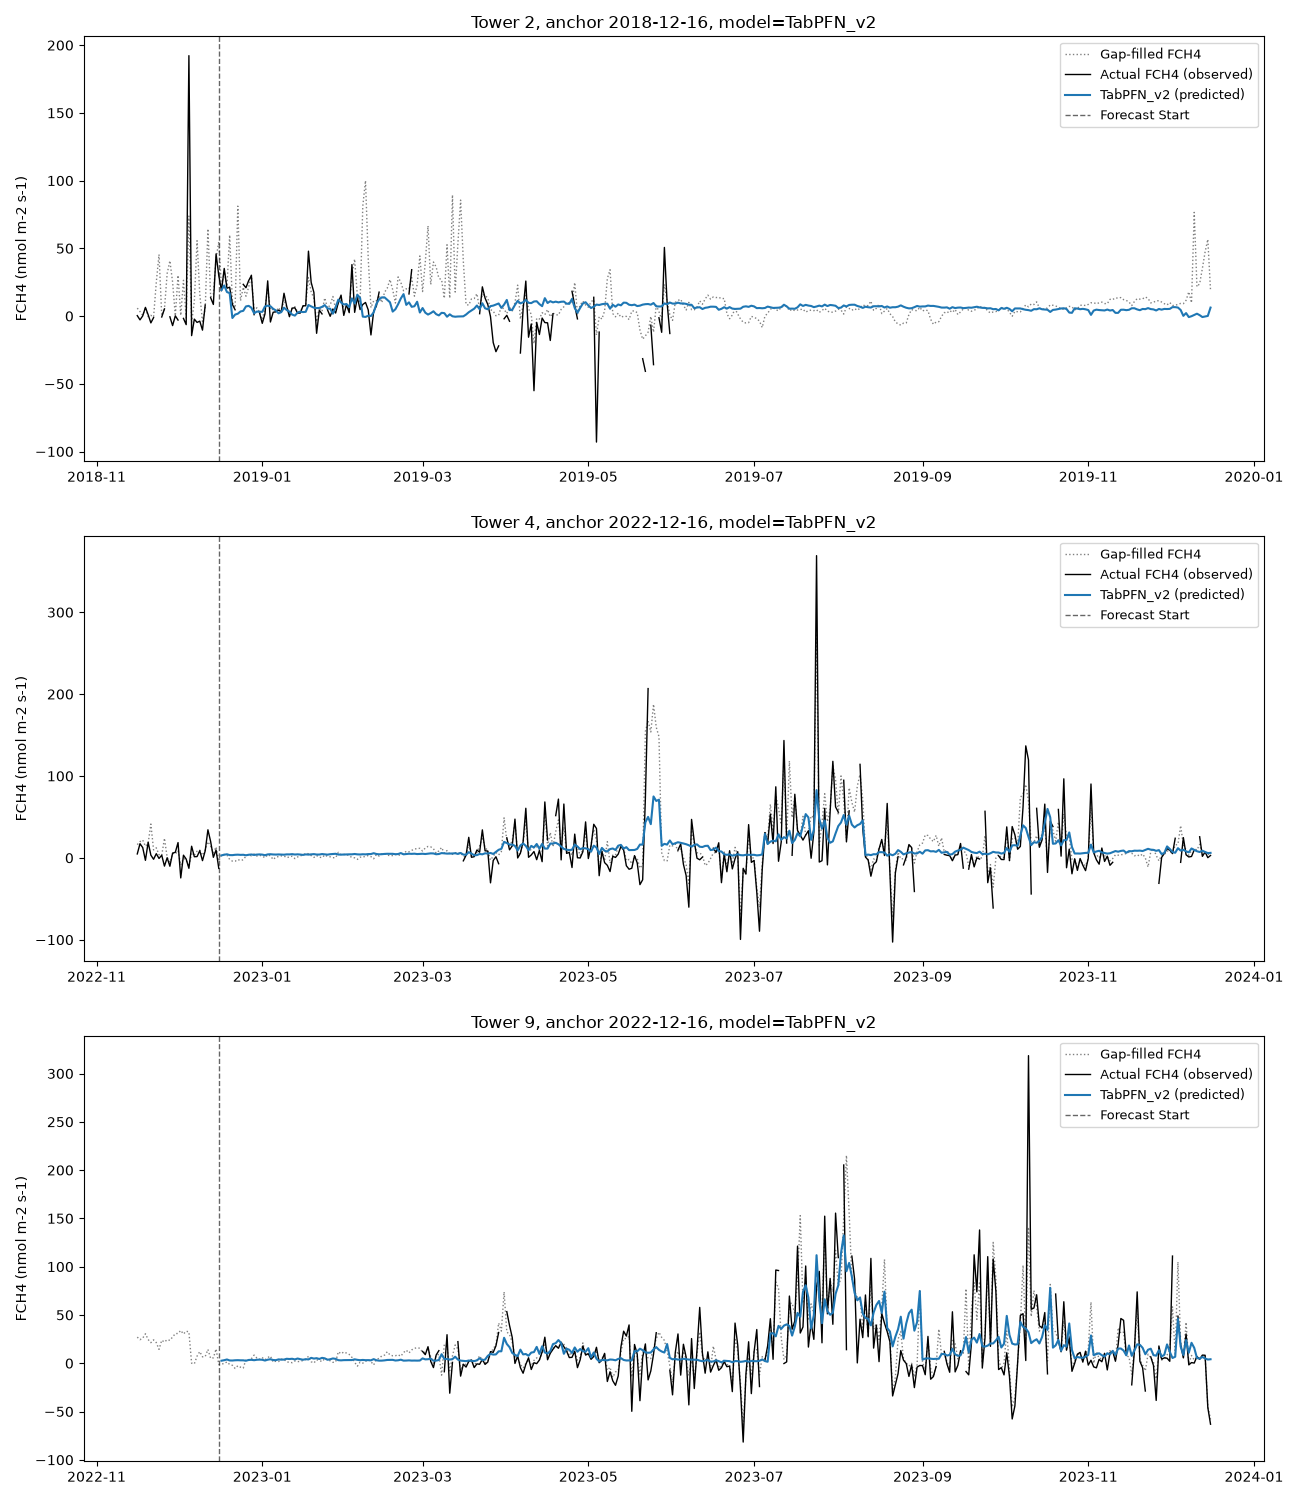
\includegraphics[width=0.85\textwidth]{Figures/ch5_champion_3towers.png}
\caption{Representative 365-day conditional forecasts from the TabPFN
model at T2, T4 and T9. The dashed vertical line marks the forecast origin;
blue lines show predictions, solid black lines show observed
FCH\textsubscript{4}, and dotted grey lines show the gap-filled series for
context.}
\label{fig:fc_champion_three_towers}
\end{figure}

\FloatBarrier

\subsection{Spike vs.\ Non-Spike Performance} \label{fc:spike}

The aggregate results conceal substantial differences between ordinary and
high-flux periods. Table~\ref{tab:fc_spike_performance} separates the
spike and non-spike observations for the TabPFN model using tower-specific
thresholds estimated exclusively from observations preceding each forecast
origin.

\begin{table}[htbp]
\centering
\footnotesize
\begin{tabular}{lcc}
\toprule
Metric & Non-spike ($n=1{,}997$) & Spike ($n=130$) \\
\midrule
MASE & 0.524 & 3.285 \\
MAE & 20.31 & 176.48 \\
RMSE & 30.01 & 210.12 \\
Bias (prediction $-$ observation) & $+1.48$ & \textbf{$-176.48$} \\
\bottomrule
\end{tabular}
\caption{Forecasting performance of the TabPFN model during non-spike and
spike periods. Spike thresholds are the tower-specific
95th percentiles estimated from pre-origin observed FCH\textsubscript{4}.}
\label{tab:fc_spike_performance}
\end{table}

Forecast errors are concentrated in the spike periods. Non-spike observations
achieved a MASE of 0.524 and MAE of 20.31, whereas spike observations reached
a MASE of 3.285 and MAE of 176.48. Bias changed from only $+1.48$ during
non-spike periods to $-176.48$ during spikes, showing that the dominant failure
is severe underprediction of high-flux events. The temporal distribution of
the evaluated spike observations is shown in Appendix
Figure~\ref{fig:app_fc_spike_timing}.

\subsection{Interpretability} \label{fc:interp}

Figure~\ref{fig:fc_tabpfn_importance} shows the permutation-sensitivity ranking for the 
TabPFN model. Livestock-unit density, total-liveweight density and cattle density occupy 
the first three positions, followed by grazing status; the remaining environmental and 
management variables have substantially smaller effects. The tower-specific rankings in 
Appendix Figure~\ref{fig:app_fc_importance_by_tower} show that this pattern is strongest 
at T4 and T9, whereas T2 relies primarily on environmental and management variables. 
Appendix Figure~\ref{fig:app_fc_importance_species} further separates the livestock 
related sensitivity by animal type.

\begin{figure}[H]
    \centering
    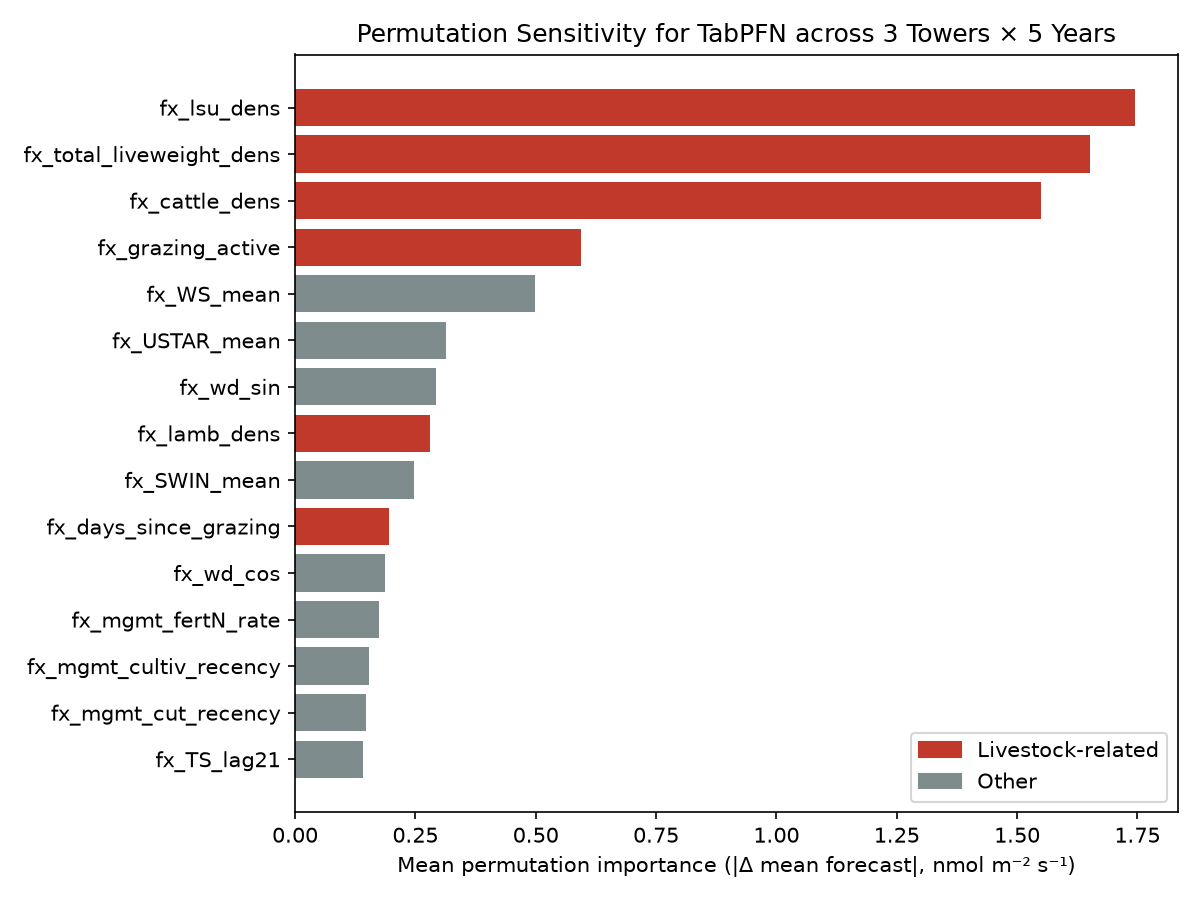
\includegraphics[width=0.8\textwidth]{Figures/ch5_tabpfn_permutation_sensitivity_overall.png}
    \caption{Permutation sensitivity of the TabPFN model, averaged across T2, T4 and T9 and five forecast origins. Each bar shows the absolute change in the mean forecast after shuffling one predictor within a tower; livestock-related variables are highlighted in red.}
    \label{fig:fc_tabpfn_importance}
\end{figure}

\subsection{Uncertainty Quantification}

Table~\ref{tab:fc_uq_by_tower} compares the raw and CQR-calibrated 90\%
prediction intervals for the TabPFN model. At T4 and T9, CQR reduced MPIW
while shifting the mild raw overcoverage to modest undercoverage: PICP changed
from 0.929 to 0.867 at T4 and from 0.928 to 0.871 at T9. T2 exhibited
substantial raw undercoverage, but its sparse
observed targets were insufficient to construct the leave-one-origin-out
calibration set. Figure~\ref{fig:fc_cqr_t4} illustrates the CQR interval
defined in Chapter~\ref{ChapModels} for T4; the corresponding T9 result is
provided in Appendix Figure~\ref{fig:app_fc_cqr_t9}. Appendix
Figure~\ref{fig:app_fc_uq_t2_raw} instead shows T2's uncalibrated raw interval.

\begin{table}[H]
\centering
\footnotesize
\begin{tabular}{lcccc}
\toprule
& \multicolumn{2}{c}{PICP} & \multicolumn{2}{c}{MPIW} \\
\cmidrule(lr){2-3}\cmidrule(lr){4-5}
Tower & Raw & CQR & Raw & CQR \\
\midrule
T2 & 0.726 & -- & 86.04 & -- \\
T4 & 0.929 & 0.867 & 187.13 & 178.14 \\
T9 & 0.928 & 0.871 & 192.84 & 186.89 \\
\bottomrule
\end{tabular}
\caption{Raw and CQR-calibrated 90\% prediction-interval performance for the
TabPFN model. PICP is the empirical
coverage proportion and MPIW is reported in
$\mathrm{nmol\,m^{-2}\,s^{-1}}$. CQR values are unavailable for T2
because too few observed targets remained to construct its calibration set.}
\label{tab:fc_uq_by_tower}
\end{table}

\begin{figure}[H]
\centering
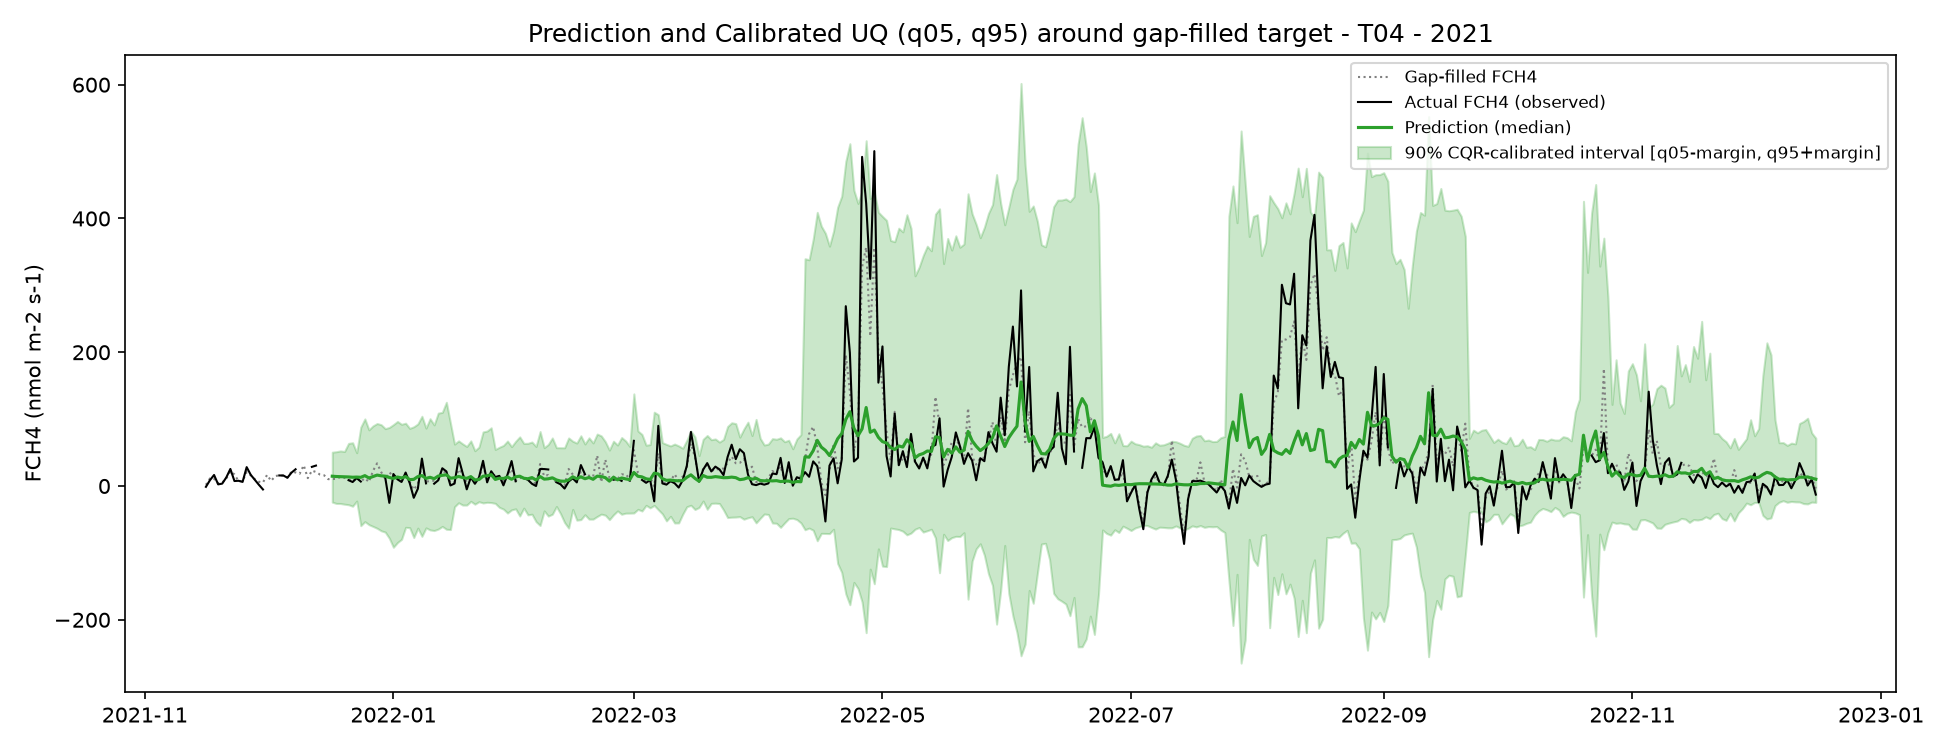
\includegraphics[width=\textwidth]{Figures/cqr_gallery/ch5_cqr_forecast_T04_2021.png}
\caption{Representative 365-day TabPFN forecast at T4 from the 2021 forecast
origin. The green line is the median forecast, the black line shows available
observations, the dotted line provides the gap-filled series as context, and
the shaded region is the 90\% CQR-calibrated prediction interval across the
complete forecast horizon. The corresponding T9 result is provided in Appendix
Figure~\ref{fig:app_fc_cqr_t9}.}
\label{fig:fc_cqr_t4}
\end{figure}

Overall, TabPFN achieved the strongest average forecasting performance, but
its errors remained concentrated during high-flux periods. Livestock-related
variables dominated its sensitivity at T4 and T9, while CQR produced modest
undercoverage and could not be applied at T2. These findings show that reliable
long-horizon forecasting remains constrained by abrupt methane dynamics and
sparse observations.
